\documentclass[a4paper,12pt]{article}

% \usepackage{report}
\usepackage{lipsum}
\usepackage[margin=1in,left=1.5in,includefoot]{geometry}
\usepackage{fancyhdr}
\usepackage[titles]{tocloft}
\usepackage{graphicx}
\usepackage[ampersand]{easylist}
\usepackage{booktabs}
 % \usepackage[refpage]{nomencl}

% Break paragraphs
\setlength{\parindent}{0pt}
\setlength{\parskip}{1.8em}


% Section heading before/after spacing
\usepackage[explicit]{titlesec}
\titlespacing{\section}{0pt}{0pt}{3em plus 0pt minus 5pt}
\titlespacing{\subsection}{0pt}{2em plus 0pt minus 5pt}{2em plus 0pt minus 5pt}
\titlespacing{\subsubsection}{0pt}{2em plus 0pt minus 5pt}{2em plus 0pt minus 5pt}
\titleformat{\section}{\bfseries\large}{\thesection.}{1em}{\MakeUppercase{#1}}
\titleformat{\subsection}{\bfseries\normalsize}{\thesubsection.}{1em}{#1}
\titleformat{\subsubsection}{\bfseries\normalsize}{\thesubsubsection.}{1em}{#1}

% Spacing before/after equations
\AtBeginDocument{
  \setlength\abovedisplayskip{1.5em plus 4pt minus 5 pt}
  \setlength\belowdisplayskip{1.5em plus 4pt minus 5 pt}
  \setlength\abovedisplayshortskip{1em plus 4pt minus 5 pt}
  \setlength\belowdisplayshortskip{1em plus 4pt minus 5 pt}
}

\begin{document}
\begin{titlepage}
  \begin{center}
    {\Huge\textsc Tribhuvan University}\\
    [0.03in]
    {\LARGE\textsc Institute of Engineering}\\
    [0.05in]
    {\Large\textsc Pulchowk campus}\\
    [0.02in]
    {\large\textsc Lalitpur, Nepal}\\
    [0.2in]
    %\line(1,0){100}\\
\begin{figure}[ht!]
  \centering
  
\includegraphics[width=100px]{figs/tu-logo.jpg}
\end{figure}
    %\normalized{\bfseries Minor Project Proposal on}\\
    {\LARGE \textsc{A Major Project Proposal on}}\\
    [0.5cm]
    % \huge{\bfseries satin - chatbot}\\
    {\Large \textsc{Personality Based \\
    Music Recommendation System}}\\
    [1.8in]
    %\line(1,0){200}\\
    
    {\LARGE\textsc{Submitted to}}\\
    [0.05in]
    {\large Department of Electronics and }\\
    {\large Computer Engineering}\\
    {\large Pulchowk Campus}\\
    [1in]

    {\LARGE \textsc{\large Submitted by}}\\
    [0.05in]
    {\large Miran Ghimire (070bct521)}\\
    [0.05in]
    {\large Nabin Bhattarai (070bct522)}\\
    [0.05in]
    {\large Abhishek Paudel (070bct502)}\\
    [0.05in]
    {\large Brihat Ratna Bajracharya (070bct513)}\\
    [0.05in]
  \end{center}
\end{titlepage}

\pagenumbering{roman}
\setcounter{page}{2}

\section*{Acknowledgement}
\addcontentsline{toc}{section}{Acknowledgement}
	We would like to express our sincere gratitude to the \textbf{Department of Electronics and Computer Engineering }of IOE, Pulchowk Campus for providing us opportunity to implement the knowledge gained over these years as the Major Project for fourth year.\\ 
	Besides we are highly indebeted to our teacher \textbf{Dr. Aman Shakya} for providing valuable suggestion, guidance and motivation for this project.\\
Finally we would also like to thank all of our friends who have directly and indireclty assisted us for selecting this project.
\cleardoublepage

\tableofcontents
\thispagestyle{empty}
\cleardoublepage


\listoffigures
\thispagestyle{empty}
\cleardoublepage

\section*{List Of Abbreviations}
\thispagestyle{empty}
CF : Collaborative Filtering\\
API : Application Programming Interface\\
TF-IDF: Term Frequency- Inverse Document Frequencya\\
NLP : Natural Language Processing\\
\cleardoublepage

\section*{Abstract}
With the evolution of internet and popularity of social media, it has become the most prominent and dominent source of information sharing and communication. A person's perference can be determined using his/her social media. Hence based on this information about his/her profile related content can be delievered to the user.\\
Therefore we have come with ``\textbf{Personality Based Music Recommendation System}''. This project mainly concentrates on the recommendation of the music based on the preference of the user which basically consists ofthe three parts as input,process and output. In input part, the system takesuser data fetched from the social media and information about the music.In the processing media, the userdata and music data are analyzed for the recommender system(content based and collaborative filtering) along with the user's personality using Big 5 Personality Traits. Similarly, in the output part, it recommends the music to the user.
\thispagestyle{empty}
\cleardoublepage
\pagenumbering{arabic}
\section{Introduction}
	``\textbf{Personality Based Music Recommendation}'' is the system to recommend the music to the users based his/her preference which is obtained from the social media. In this contemporary era of digital technologies, social media has become one of the prominent means for information sharing and communication. Likewise music has been one of the prominent market of entertainment. People listen to music everyday. The fact that music can blend with any emotion has made it's way to different sorts of people with different sorts of personality.\\
	Hence we have come up with the system to recommend the music to a different people based on their social media profiles.Previous work has shown that the information in users social media profiles is reflective of their actual personalities, not an idealized version of themselves, which makes social media platform for studying a people personality.\\
	Several well studied personality models have been proposed, among which the Big Five model is established as the most popular one,which suggests that the regularity in someone's behavior over time and situations uniquely identifies his/her personality type along five dimesions: Openness to experience, Neuroticsm, Extroversion, Aggreableness and Conscientiousness.
\cleardoublepage

\section{Feasibility Study Report}
	Feasibility of the project has been sub-divided into the further three components and are presented as:\\
	\subsection{Operational Feasibility}
	Since the end product is a website to recommend music to the user based on their social profiles, the proposed system requires the use of internet which are readily available across many countries. Hence the proposed system is operationally feasible.
	\subsection{Technical Feasibility}
	As the technical specification of the software is a computer and internet which are readily available along with the data(music and social media profiles), our system is technically feasible.
	\subsection{Economic Feasibility}
	After the cost analysis of the system regarding the implementation cost, technical cost we can conclude the system is economically feasible as well.
\cleardoublepage

\section{Objective of the Project}
The primary objective of the project is to design, develop and implement a fully functional system to recommend user the music based on his/her social media profile. The whole process of creating system is intended to be achieved through a series of minor procedures, which can be further subdivided into two major stages.\\
The first involved the problem study, solution proposition, designing, developement and system installation. The second phase include the acutal operation, solution of obsolescence problems and progress toward the new standards.\subsection{Stage 1}
\begin{itemize}
	\item To make it easier for social media user to get information about musci based on their personal preference.
	\item To design and implement simple, informative and easy to use user interface.
	\item To design and develope the system according to the people's need using the latest available technology.
\end{itemize}
\subsection{Stage 2}
\begin{itemize}
	\item To implement the system for the access to the real world.
	\item Consolidating the sytem by removing the trival features and small as well as big bugs.
	\item Removing the obsolescene problems.
	\item To revise the system according to the need and change of standard in use.
\end{itemize}

\cleardoublepage

\section{Literature Review}
\subsection{Big Five Model of Personality Dimensions}
The Big Five model of personality dimensions has emerged as one of the well-researched and well-regarded measures of personality structure in recent years. The models encorporates the five domain of personality: Openess, Conscientiouness, Extroversion. Agreeableness, and Neuroticism,were conceived by Tupes and Christal as the fundamental traits that emerged from the analysis of the pervious personality tests. McCrae, Costa and John continued five factor model research and consistently found generality across age, gender and clultural lines. The Big Five traits are characterized by the following:
\begin{itemize}
	\item \textbf{Openness to Experience:} curious, intelligent, imaginative. High scorers tend to be artistic and sophisticated in taste and appreciate diverse views, ideas and experiences.
	\item \textbf{Conscientiousness:} responsible, organized, preservering. Conscientious individuals are extremely realiable and tend to be high achievers, hard workers and planners.
	\item \textbf{Extroversion:} outgoing, amicable, assertive. Friendly and energetic, extroverts draw inspiration from social situations.
	\item \textbf{Agreeableness:} cooperative, helpful,nurturing. People who score high in agreeableness are peace-keepers who are generally optimistic and trusting of others.
	\item \textbf{Neuroticism:} anxious, insecure, sensitive. Neurotics are moody, tense and easily tipped into experiencing negative emotions.
\end{itemize}

\subsection{Proposed System}
	The proposed system will be able to recommend the music to the user based on their social media profiles, saving the actual precious time of the users for searching the music of their choice. We have proposed a system that bascially has the following features:
\begin{itemize}
	\item Recommendation of the music based on the social media profile.
	\item Elimination of the search for the right music.
	\item Provision for the easy access to music.
	\item Personality analysis of the users based on social media profiles.
\end{itemize}
\subsection{Project Description}
The proposed system provides the user with the recommendation of the music bbased on the social media profiles replacing the conventional method of seraching the music of the right chocie.
Our sytem comprises of the two yet interdependent subsystems.
\begin{itemize}
	\item Front End \\
		It is the visible part of the system. The user will interact with this part of the system. It offers the GUI for the interaction and consists of login, recommedation of music based on the social media profile.
	\item Back End \\
		This is the part of the system where all user and music items profiles are stored. Every processing work that is to be done will be done by the back end of the system. This unit is handled by the admin/developers who are responsible for the addition, modification, updating the content of the system.
\end{itemize}
\cleardoublepage

\section{Methodology}

\subsection{Design Approach}
The proposed system is intended to be developed with the \textbf{``Incremental Developement Approach''}. Thus proposed system is expected to be evolved through the several versions until complete system has been developed interleaving the activity of specification, developement and validation.
\begin{figure}[ht!]
  \centering
  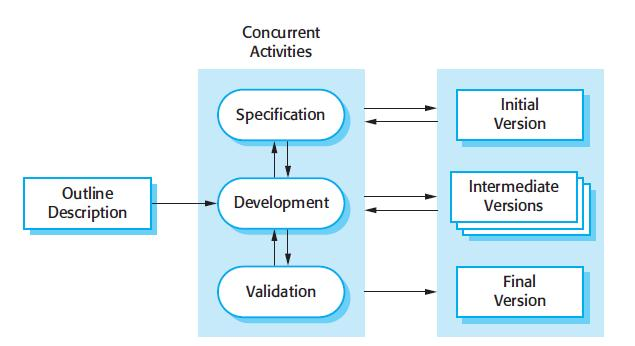
\includegraphics[width=450px]{figs/incremental.jpg}
  \caption{Incremental Development Approach \label{fig:incremental}}
\end{figure}

\subsection{Primary/Secondary Source of Data Collection}
The data set used in our system are:
\begin{enumerate}
\item User's profile\\
  It will be extracted from facebook API and ``myPersonality'' dataset will be used to study the personality of the users with the help of their online profile features and status update text.
\item Music data set\\
  It will be extracted from Million Song Dataset from kaggle. \\
  Available Features of Music data set are :
  \begin{enumerate}
  \item List of Artist and Titles
  \item Track-level tags and similar tracks
  \item Music Lyrics
  \end{enumerate}
\end{enumerate}

\subsection{System Block Diagram}
\begin{figure}[ht!]
  \centering
  \includegraphics[width=400px]{figs/pbrs.png}
  \caption{System Block Diagram \label{fig:pbrs}}
\end{figure}
i
\subsection{Algorithm to be used}
\subsubsection{Personality Deduction}
Personality of the user will be deduced using Big Five model of personality dimensions which will be done in the following ways:
\begin{itemize}
\item \textbf{Feature Extraction:} Dataset provided by the ``mypersonality''will used to study the personality of the facebook users. Dataset consists of survey of facebook users to study a their personality traits. The feature extraction will be done using \textbf{``Text Classification''} on the dataset using NLP and the feature set will be a \textbf{``Bag of words''} that can describe the personality traits of the users. It can furthur be optimized wwith TF/IDF analysis.
\item \textbf{Classification Algorithm:} As Naive Bayes classification provides the probabilistic view on the classification items based on the given sets of input, we will be using Naive Bayes algorithm to predict the personality on probability basis.\\
	Overfitting,Underfitting and efficency will be solved with cross-validation,log space and tf-idf model.
	Besides, other classification alogrithms such as logistic regression,SVM can be applied to a problem as well.
\end{itemize}
\subsubsection{Music Recommendation System}
We are planning to use Hybrid Recommendation Algorithm which comprises of Content, Collaborative Recommendation Algorithm.
\begin{itemize}
\item Content Based Recommendation System :\\
  In this system, the features set are extracted from the content (Music data), which in turn are used for the recommendation.
\item Collaborative Filtering :\\
  In this system patterns of user behavior/model are observed for the recommendation.
\end{itemize}
Besides as the lyrics of the song is provided within the ``Million Song Dataset'', NLP(Text classification) can be applied to the lyrics in order to determine it's emotion which can be applied to recommend the music to the user based on his/her personality.
\cleardoublepage

\subsection{Algorithm Flow Diagram}
\begin{figure}[ht!]
  \centering
  \includegraphics[width=100px]{figs/algoflow.png}
  \caption{Algorithm Flow Diagram \label{fig:algoflow}}
\end{figure}

\subsection{Description of each block/module}

\begin{enumerate}
\item User Model\\
  The User's information will be extracted from facebook profile. The extracted information will be used to create a user's model i.e personality prediction using Big 5 personality traits.
\item Feature Extraction\\
  Required features are extracted from Music data-set. These features will be used to classify the music data.
\item Recommendation System\\
  Using User Model and Feature Extraction module, using algorithm mentioned above we can recommend appropriate music to a user.
\item Error Correction\\
  The Error Correction module is used to increase the efficiency and accuracy of Recommendation system. Using the feedback of user we can modify the User's Model.
\end{enumerate}
\cleardoublepage


\subsection{Requirement List (Hardware/Software Tools)}
Hardware Requirements :
\begin{itemize}
\item Server Specifications
  \begin{itemize}
  \item Minimum internal Memory 16GB
  \item 1 TB secondary Memory
  \end{itemize}
\item Power Backup System for emergency power cut
\end{itemize}

Software Tools :
\begin{itemize}
\item Apache Web Server Application
\item Python (version $>$ 3.5)
\end{itemize}

\subsection{Cost Estimation}
Hardware Cost Estimation
\begin{itemize}
\item Domain Registration : \$30 / year
\item Server Hosting : \$50 / month
\end{itemize}

\subsection{Time Schedule Estimation}
\begin{figure}[ht!]
  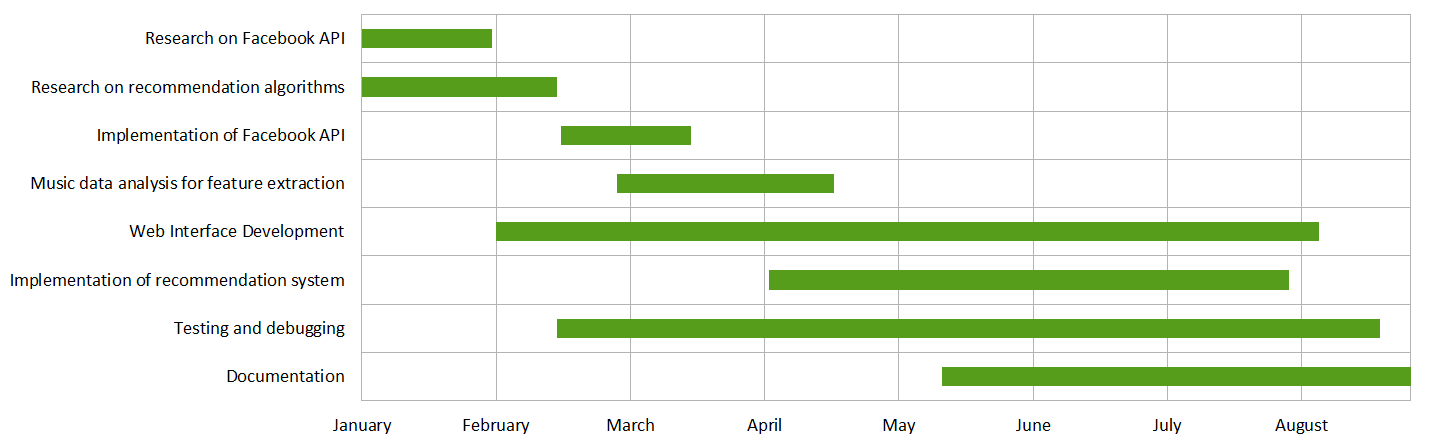
\includegraphics[width=450px]{figs/ganttchart.png}
  \caption{Time Estimation Using Gantt-Chart \label{fig:ganttchart}}
\end{figure}

\subsubsection{Part A: Proposal to Mid-Term Defense}
According to our Gantt-chart, till mid-term we are going to complete user model, feature extraction from music and simple web-interface front-end.
\subsubsection{Part B: Mid-Term to Final Presentation}
\begin{itemize}
\item Implementation of Recommendation system
\item Web-Interface
\item Testing and Debugging 
\item Documentation.
\end{itemize}

\section{Expected Outcomes/Result}
The system is expected to recommed the music to the social media users based on their's proiles.
\subsection{Achievements and Benefits}
\begin{itemize}
\item The major advantage the people will receive from the system is the easy access to the right music of their choice eliminating the conventional method of searching the right music. It makes easier to get right music according to their taste for users.
\item This is system is supposed to save user's time for the search of music of their taste.
\end{itemize}
\cleardoublepage

\section{Present Scope and Future Improvement}
\subsection{Present Scope}
The most important scope of this project will be to act as a prototype to recommend music to the social media users based on their profiles.
\subsection{Future Improvement}
The major enhancement that can be done to a system can be acheived by making the system \textbf{``Feed Recommendation System''}. The feed might include the movies,sports, news, weather news etc.\\
Moreover, the system can be benefical to the other recommendation system like e-commerce,movie streaming channels whereby user's behavior is critical on to recommend the other product.\\
Besides the system can also have the mobile application to interact with the system as smartphones are popular these days.
\cleardoublepage

\section{Conclusion}
Thus after the completion of the project, we will be able to make a recommendation system to the social media users based on their profiles eliminating the conventional method of searching the music of the choice as well as predict his/her personality based on his/her social media account.
\cleardoublepage

%\bibliographystyle{ieeetr}
%\addcontentsline{toc}{section}{\numberline{}References}
%\bibliography{proposal}
%\nocite{*}
\addcontentsline{toc}{section}{References}
\begin{thebibliography}{9}
	\bibitem{myPersonality DataSet}
		myPersonality DataSet,
	\\\texttt{http://mypersonality.org/wiki/doku.php}
	\bibitem{Million Song DataSet}
		Kaggle:Your Home for Data Science
	\\\texttt{https://labrosa.ee.columbia.edu/millionsong}
	\bibitem{NLP}
	Christopher Manning,Stanford NLP-Stanford NLP Group
	\\\texttt{https://nlp.standford.edu/manning/}
	\bibitem{Recommendation System}
	Recommendation System,Courseera,
	\\\texttt{https://coursera.org/learn/machine-learning}
	\bibitem{Big 5 Personality Traits}
	Studying the big five personality traits-UK Essays,
	\\\texttt{https://ukessays.com/essays/psychology/studying-the-big-five-personality-traits.php}
\bibitem{Facebook Graph API}
	Facebook Graph API,
	\\\texttt{https://developers.facebook.com/docs/graph-api}
\end{thebibliography}
\end{document}
